% !TEX encoding = UTF-8 Unicode
% !TEX root = ../thesis.tex


%
%\section{Overview}
%In this paper, we present two human body prior models for total body motion capture. 
%% The major reason of presenting two models is the fact that we need a way to accurately reconstruct total body shape and motion first in order to build a new model learnt from the data, which is a chicken and egg problem.  
%%Instead of building the desired body model from the scratch,
%We first present the ``Frankenstein model" to consolidate existing high-quality part models (face, body, and hands) into a single skeleton hierarchy. Capturing shape and motion of the total body is then possible by fitting the Frankenstein model to 3D sensor measurements, including 3D keypoints and 3D point clouds. We find that total motion capture with the Frankenstein model already produces compelling results, as shown in the accompanying video. However, there are several aspects that need improvement: (1) the model only produces shapes without hair and clothing; (2) model optimization is complex, and requires additional optimization parameters to keep the parts connected without artifacts, making implementation complicated; and (3) the definition of joints for the 2D detectors is different from the actual location of the joints in the 3D skeleton, resulting in a nonzero cost function even for the correct pose.
%
%To this end, we present a model, named ``Adam", aiming to capture total body motion with a simpler parameterization. The model is built from the reconstruction data leveraged by the Frankenstein model for various motions of 70 subjects. Since the reconstruction data has diversity in clothings and hairs, the learned linear subspace model of Adam has a degree of expressive power for hairs and clothing. 
%
%Finally, we evaluate our method on various challenging sequences captured in the CMU Panoptic Studio~\cite{Joo-15}.

%
%\subsection{Discussion}
%\label{Franken:discussion}
%We find that total motion capture with the Frankenstein model already produces compelling results, as shown in the accompanying video. However, there are several aspects which need improvements: 1) the model only produces shapes without hairs and clothing, very different from the natural interactions we aim to capture; 2) model optimization is complex, and requires additional optimization parameters to keep the parts connected without artifacts, making implementation complicated, and 3) the definition of joints for the 2D detectors is different from the actual location of the joints in the 3D skeleton, resulting in a nonzero cost function even for the correct pose.

%

% \begin{figure}[t]
% 	%	\includegraphics[width=0.49\columnwidth]{fig/smpl_parts_aligned_3}
% 	%	\includegraphics[width=0.49\columnwidth]{fig/totalmesh_3}
% 	%\includegraphics[width=\columnwidth]{totalmodelbuilding4}
% 	\includegraphics[width=0.9\columnwidth]{Partmodels_180326.pdf}
% 	\caption{Part models and the Frank model. (a) The body model~\cite{Loper2015}; (b) the face model~\cite{cao2014facewarehouse}; and (c) a hand rig. In (a-c), the red dots have corresponding 3D keypoints reconstructed by detectors.} %(d) Aligned face and hand models (gray meshes) to the body model (the blue wireframe mesh); and (e) the seamless Frank model.}
% 	\label{fig:frankenstein_part_aligned}
% 	%	\label{fig:frankenstein_mesh}
% 	% Yaser: (d) and (e) as a separate figure
% \end{figure}

\begin{figure}[t]
	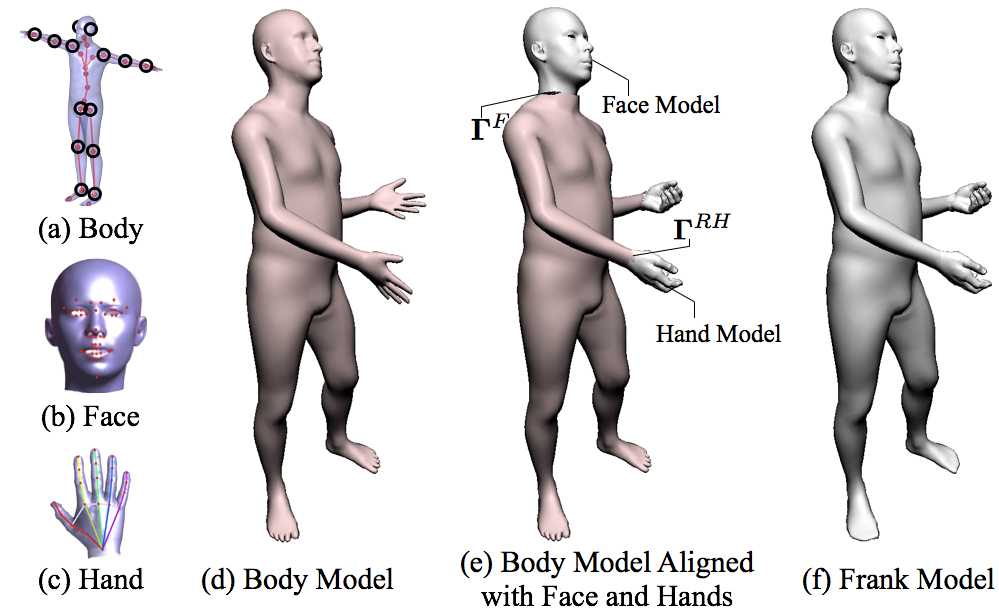
\includegraphics[trim={1cm 0 0 0 }, width=\columnwidth]{tbc_figures/building_frank_3}
	\caption{Part models and the Frank model. (a) The body model~\cite{Loper2015}; (b) the face model~\cite{cao2014facewarehouse}; and (c) a hand rig. In (a-c), the red dots have corresponding 3D keypoints reconstructed by detectors; (d) Body only model; (e) Face and hand models substitute the corresponding parts of the body model. Alignments are ensured by  $\bm{\Gamma}$s; and (f) The blending matrix $\mathbf{C}$ is applied to produce a seamless mesh.} %(d) Aligned face and hand models (gray meshes) to the body model (the blue wireframe mesh); and (e) the seamless Frank model.}
	\label{fig:frankenstein_part_aligned}
	%	\label{fig:frankenstein_mesh}
	% Yaser: (d) and (e) as a separate figure
\end{figure}

\section{Frank Model}

The motivation for building the Frank\footnote{Frank is an homage to a certain \emph{Modern Prometheus}.} body model is to leverage existing part models: SMPL~\cite{Loper2015} for the body, FaceWarehouse~\cite{cao2014facewarehouse} for the face, and an artist-defined hand rig (shown in Fig.~\ref{fig:frankenstein_part_aligned}). Each of these capture shape and motion details at an appropriate scale for the corresponding part.
%Thus, we have a coarser mesh for the body torso and limbs, and more detailed meshes for the face and the hands. 
This choice is not driven merely by the free availability of the component models: note that due to the trade-off between image resolution and field of view of today's 3D scanning systems, scans used to build detailed face models will generally be captured using a different system than that used for the rest of the body.
%In the near future, it is therefore likely that full-body models will be constructed by merging more detailed component models. 
For our model, we merge all transform bones into a single skeletal hierarchy but keep the native parameterization of each component part to express identity and motion variations. As the final output, the Frank model produces motion parameters capturing the total body motion of humans, and generates a seamless mesh by blending the vertices of the component meshes. 

\subsection{Stitching Part Models}

The Frank model $M^U$ is parameterized by motion parameters $\boldsymbol{\theta}^U$, shape (or identity) parameters $\boldsymbol{\phi}^U$, and a global translation parameter $\mathbf{t}^U$,
\begin{align}
\mathbf{V}^U = M^U (\boldsymbol{\theta}^U, \boldsymbol{\phi}^U, \mathbf{t}^U ),
\end{align}
where $\mathbf{V}^U$ is a seamless mesh expressing the motion and shape of the target subject.  The motion and shape parameters of the model are a union of the part models' parameters:
\begin{align}
\boldsymbol{\theta}^U = \{ \boldsymbol{\theta}^B, \boldsymbol{\theta}^F, \boldsymbol{\theta}^{LH}, \boldsymbol{\theta}^{RH}  \}, \\
\boldsymbol{\phi}^U = \{ \boldsymbol{\phi}^B, \boldsymbol{\phi}^F, \boldsymbol{\phi}^{LH},  \boldsymbol{\phi}^{RH}  \},
%\mathbf{t}^U_t = \{ \mathbf{t}^B_t, \mathbf{t}^F_t, \mathbf{t}^{LH}_t, \mathbf{t}^{RH}_t  \}
\end{align}
where the superscripts represent each part model: $B$~for the body model, $F$ for the face model, $LH$ for the left hand model, and $RH$ for the right hand model. Each of the component part models maps from a subset of the above parameters to a set of vertices, respectively, $\mathbf{V}^B \,{\in}\, \mathds{R}^{N^B{\times}3}$, $\mathbf{V}^F \,{\in}\, \mathds{R}^{N^F{\times}3}$, $\mathbf{V}^{LH} \,{\in}\, \mathds{R}^{N^H{\times}3}$, and $\mathbf{V}^{RH} \,{\in}\, \mathds{R}^{N^H{\times}3}$, where the number of vertices of each mesh part is $N^B{=}6890$, $N^F{=}11510$, and $N^H{=}2068$. The final mesh of the Frank model, $\mathbf{V}^U {\in} \mathds{R}^{N^U{\times}3}$, is defined by linearly blending them with a matrix $\mathbf{C} \in \mathds{R}^{N^U\times(N^B{+}N^F{+}2N^H)}$: 
\begin{align}
\mathbf{V}^U = \mathbf{C} 
\left[
\begin{array}{c}
\left({\mathbf{V}^B}\right)^T
\left({\mathbf{V}^F}\right)^T
\left({\mathbf{V}^{LH}}\right)^T
\left({\mathbf{V}^{RH}}\right)^T
\end{array} 
\right]^T,
\end{align}
where $T$ denotes the transpose of a matrix. Note that $\mathbf{V}^U$ has fewer vertices than the sum of part models because there are redundant parts in the body model (e.g., face and hands of the body model). In particular, our final mesh has $N^U{=}18540$ vertices. 
%If we separate Fig. 2. <--- look at Yaser's notes here
Fig.~\ref{fig:frankenstein_part_aligned} (e) shows the part models that are aligned, and (f) shows the final mesh topology of the Frank model after applying the the blending matrix $\mathbf{C}$ at the mean shape in the rest pose. 
%We define the mesh topology (vertex locations and faces) such that the boundary regions among parts are as seamless as possible. 
The blending matrix $\mathbf{C}$ is a very sparse matrix; most rows have a single column set to one with zeros elsewhere and simply copy the vertex locations from the corresponding part models with minimal interpolation at the seams.

%
%\begin{figure}[t]
%	\includegraphics[width=\columnwidth]{fig/C_mat_vis_}
%	\caption{C matrix to fuse output of part models. Showing block kind of structure of the matrix}
%	\label{fig:Total body fusion  matrix}
%\end{figure}
In the Frank model, all parts are rigidly linked by a single skeletal hierarchy, which is crucial as an output of motion capture. This unification is achieved by substituting the hands and face branches of the SMPL body skeleton with the corresponding skeletal hierarchies of the detailed part models. All parameters of the Frank model are jointly optimized for motion tracking and identity fitting. The parameterization of each of the part models is detailed in the following sections.
%, and then the joint optimization method for total body motion tracking with Frankenstein model is presented. 


%\begin{figure}[t]
%	\centering
%	%\includegraphics[width=\linewidth,clip=true,trim=60pt 0pt 0pt 0pt]{figures/fullbody/smpl_correspond}
%	\includegraphics[width=\linewidth]{figures/fullbody/smpl_correspond}
%	\caption{(a)~SMPL model~\cite{Loper2015}, template shapes (male and female) and first two basis vectors of shape variation. (b)~SMPL model joint hierarchy. Joints or vertices with a direct correspondence to a detected point are circled. (c)~2D detections corresponding to the outlined joints.\label{fig:smpl_correspond}} 
%\end{figure}



\subsection{Body Model}

For the body, we use the SMPL model~\cite{Loper2015} with minor modifications. 
%The SMPL model is a principal component analysis (PCA) based model of body shape that is deformed via linear blend skinning and pose-dependent corrective blendshapes. 
In this section, we summarize the salient aspects of the model in our notation. The body model, $M^B$, is defined as follows,
\begin{align}
\mathbf{V}^B = M^B (\boldsymbol{\theta}^B, \boldsymbol{\phi}^B, \boldsymbol{t}^B ),
\end{align}
with $\mathbf{V}^B = \{ \mathbf{v}^B_i\}_{i=1}^{N^B}$. 
The model uses a template mesh of $N^B{=}6890$ vertices, where we denote the $i$-th vertex as $\mathbf{v}^B_i\in\mathds{R}^3$. 
% The vertices of this template mesh are first displaced by a set of blendshapes describing the {\em identity} or body shape, yielding mesh vertices $\hat{\mathbf{v}}^B_i$ in the rest shape,
% \begin{align}
% \hat{\mathbf{v}}^B_i = \mathbf{v}^{B0}_i + \sum_{k=1}^{K_b} \mathbf{b}^k_{i} \phi^B_k,
% \label{eq:smpl_shape_coeffs}
% \end{align}
% where $\mathbf{b}^k_{i}\in\mathds{R}^3$ is the $i$-th vertex of the $k$-th blendshape, $\phi^B_k$ is the $k$-th shape coefficients of $\mathbf{\phi^B}\in\mathds{R}^{K_b}$, $K_b=10$ is the number of identity body shape coefficients, and $\mathbf{v}^{B0}_i$ is the $i$-th vertex of the mean shape.
% Given the vertices in the rest pose, the posed mesh vertices are obtained by linear blend skinning using transformation matrices $\mathbf{T}_j\in\mathds{R}^{4\times 4}$ for each of the $J$ joints,
% \begin{align}
% \mathbf{v}_i^B= \mathbf{I}_{3\times 4} \cdot \sum_{j=1}^{J^B} w_{i,j}\mathbf{T}^B_j (\theta^B) \begin{pmatrix} \hat{\mathbf{v}}^B_i \\ 1 \end{pmatrix},
% \label{eq:full_lbs_pose}
% \end{align}
% where the transformation matrices $\mathbf{T}_j$ encode the transform for each joint $j$ from the rest pose to the posed mesh in world coordinates, which is constructed by following skeleton hierarchy from the root joint. The $j$-th pose parameter $\boldsymbol{\theta}_j$ is the angle-axis representation of the relative rotation of joint $j$ with respect to its parent joints. $w_{i,j}$ is the weight with which transform $\mathbf{T}_j$ affects vertex $i$, with $\sum_{j=1}^Jw_{i,j}{=}1$ and $\mathbf{I}_{3\times 4}$ is the $3{\times} 4$ truncated identity matrix to transform from homogenous coordinates to a $3$ dimensional vector. We use $J^B{=}21$ with $\theta^B \,{\in}\, \mathds{R}^{21{\times}3}$, ignoring the last joint of each hand compared to the original SMPL model. For simplicity, we do not use the pose-dependent blendshapes during fitting.
The vertices of this template mesh are first displaced by a set of blendshapes describing the {\em identity} or body shape. Given the vertices in the rest pose, the posed mesh vertices are obtained by linear blend skinning (LBS) using transformation matrices $\mathbf{T}^B_j\in \textrm{SE(3)}$ for each of the $J$ joints,
\begin{align}
\mathbf{v}_i^B= \mathbf{I}_{3\times 4} \cdot \sum_{j=1}^{J^B} w^B_{i,j}\mathbf{T}^B_j\begin{pmatrix} \mathbf{v}^{B0}_i + \sum_{k=1}^{K_b} \mathbf{b}^k_{i} \phi^B_k \\ 1 \end{pmatrix},
\label{eq:full_lbs_pose}
\end{align}
where $\mathbf{b}^k_{i}\in\mathds{R}^3$ is the $i$-th vertex of the $k$-th blendshape, $\phi^B_k$ is the $k$-th shape coefficient in $\boldsymbol{\phi}^B\in\mathds{R}^{K_b}$ with $K_b{=}10$ the number of identity body shape coefficients, and $\mathbf{v}^{B0}_i$ is the $i$-th vertex of the mean shape. The transformation matrices $\mathbf{T}^B_j$ encode the transform for each joint $j$ from the rest pose to the posed mesh in world coordinates, which is constructed by traversing the skeleton hierarchy from the root joint with pose parameter $\boldsymbol{\theta}^B$ (see~\cite{Loper2015}). The $j$-th pose parameter $\theta^B_j$ is the angle-axis representation of the relative rotation of joint $j$ with respect to its parent joints. $w^B_{i,j}$ is the weight with which transform $\mathbf{T}^B_j$ affects vertex $i$, with $\sum_{j=1}^{J^B}w^B_{i,j}{=}1$ and $\mathbf{I}_{3\times 4}$ is the $3{\times} 4$ truncated identity matrix to transform from homogeneous coordinates to a $3$ dimensional vector. We use $J^B{=}21$ with $\boldsymbol{\theta}^B \,{\in}\, \mathds{R}^{21{\times}3}$, ignoring the last joint of each hand of the SMPL model. For simplicity, we do not use the pose-dependent blendshapes\footnote{For our target sequences, the modeling error between the SMPL model~\cite{Loper2015} and the 3D surface measurements is dominated by clothing artifacts, which the pose-blendshapes were not trained on.}.
%While the original SMPL model has $J^B{=}24$ with $23$ joints and an additional root transform to orient the body in world-space coordinates, we omit the last joint of each hand, and use $J^B{=}21$ with $\theta^B \,{\in}\, \mathds{R}^{21{\times}3}$. For simplicity, we do not use the pose-dependent blendshapes during fitting; this results in faster optimization runtimes and a sparser Jacobian matrix during the minimization.
% Additionally, we use only the male model as we will deform the surface to match each person's surface.

% The transformation matrices $\mathbf{T}_j$ encode the transform for each joint $j$ from the rest pose to the posed mesh in world coordinates, and are a function of the joint angles $\boldsymbol{\theta}\in\mathds{R}^{3\times J}$ (including the world-space orientation of the body) and the world-space translation $t \in\mathds{R}^3$. Each column $\boldsymbol{\theta}_j$ is the angle-axis representation of the relative rotation of joint $j$ with respect to its parent joint. A key characteristic of the SMPL model is that these transformations also depend on the shape coefficients $\mathbf{a}$; we refer the reader to~\cite{Loper2015} for details on the construction of these matrices. Let us call $\mathbf{V}_b{=}[\mathbf{v}_1 \dots \mathbf{v}_V]\in\mathds{R}^{3\times V}$ the full set of posed vertices in world coordinates. We can then compose the action of Eq.~\eqref{eq:smpl_shape_coeffs} and Eq.~\eqref{eq:full_lbs_pose} into a function that transforms from the set of body parameters (body shape $\mathbf{a}$, body pose $\boldsymbol{\theta}$, and translation $\mathbf{t}$) to the posed vertices of the body mesh in world coordinates,
%\begin{align}
%\mathbf{V}_b = b( \mathbf{a}, \boldsymbol{\theta}, \mathbf{t} ).
%\end{align}
%Fig.~\ref{fig:smpl_correspond}a shows the vertices of the SMPL model in its rest pose, color coded to illustrate the region of influence of each bone. Each color corresponds to a different bone, and the smooth blending between colors reflects the changing relative weights of each of the bones influencing a single vertex. Fig.~\ref{fig:smpl_correspond}b shows the full joint hierarchy, which at $23$ joints is more complex than the subset of joints detected (Fig.~\ref{fig:smpl_correspond}c) and triangulated (Fig.~\ref{fig:smpl_correspond}d) by the method of Sect.~\ref{sect:markerless_mocap}. Note that the detected points do not cover all degrees of freedom captured by the SMPL model, particularly details about body shape as well as the orientation of certain limbs, notably the forearms, head, and feet.

\subsection{Face Model}
\label{subsection:face}
As a face model, we build a generative PCA model from the FaceWarehouse dataset~\cite{cao2014facewarehouse}. Specifically, the face part model, $M^F$, is defined as follows,
\begin{align}
\mathbf{V}^F = M^F (\boldsymbol{\theta}^F, \boldsymbol{\phi}^F, \mathbf{T}^F ),
\end{align}
with $\mathbf{V}^F = \{ \mathbf{v}^F_i\}_{i=1}^{N^F}$, where the $i$-th vertex is $\mathbf{v}^F_i\in\mathds{R}^3$, and $N^F{=}11510$. The vertices are represented by combining shape and expression subspaces:
%The model uses a template mesh of $N^F{=}11510$ vertices, where we denote the $i$-th vertex as $\mathbf{v}^F_i\in\mathds{R}^3$. We decompose the shapes in the dataset into two linear subspaces, one corresponding to identity and one corresponding to expression variations. The $i$-th face vertex is represented by the linear combination of the subspaces:
\begin{align}
\hat{\mathbf{v}}_i^F = \mathbf{v}^{F0}_i + \sum_{k=1}^{K_{f}} \mathbf{f}^k_{i} \phi^F_k  + \sum_{s=1}^{K_{e}} \mathbf{e}^s_{i} \theta^F_s
\label{eq:face_shape}
\end{align}
where, as before, $\mathbf{v}^{F0}_i$ denotes $i$-th vertex of the mean shape, and $\phi^F_k$ and $\theta^F_s$ are the $k$-th face identity (shape) and $s$-th facial expression (pose) parameters respectively. Here, $\mathbf{f}^k_i\in\mathds{R}^3$ is the $i$-th vertex of the $k$-th identity blendshape ($K_{f}=150$), and $\mathbf{e}^s_i\in\mathds{R}^3$ is the $i$-th vertex of the $s$-th expression blendshape ($K_{e}=200$). 

Finally, a transformation $\mathbf{T}^F$ brings the face vertices into world coordinates. To ensure that the face vertices transform in accordance to the rest of the body, we assume that the mean face $\mathbf{v}^{F0}_i$ is aligned with the body mean shape as shown in Fig.~\ref{fig:frankenstein_part_aligned}, which is manually done in building the model. This way, we can apply the transformation of the body model's head joint $\mathbf{T}^B_{j=F}(\boldsymbol{\theta}^B)$ as a global transformation for the face model in Eq.~\ref{eq:face_pose}. However, to keep the face in alignment with the body, an additional transform matrix $\bm{\Gamma}^F \in \textrm{SE(3)}$ is required to compensate for displacements in the root location of the face joint due to body shape changes in Eq.~\ref{eq:full_lbs_pose}. 

Finally, each face vertex position is given by:
\begin{align}
\mathbf{v}^F_i = \mathbf{I}_{3\times 4} \cdot \mathbf{T}^B_{j=F} \cdot \bm{\Gamma}^F \begin{pmatrix} \hat{\mathbf{v}}^F_i \\ 1 \end{pmatrix},
\label{eq:face_pose}
\end{align}
where the transform $\bm{\Gamma}^F$, which is directly determined by the body shape parameters $\boldsymbol{\phi}^B$, aligns the face model with the body model.

%\subsection{Hand Model}
%We use an artist rigged hand mesh. Our hand model has $J^H{=}16$ joints and, similarly to the body model, the mesh is deformed via linear blend skinning. The hand model has a fixed shape, but we introduce scaling parameters to allow for different finger sizes by adding $X$,$Y$, and $Z$ scaling factors to each bone. The left hand and right hand models are exactly the same (but reflected), so we refer to either of them as H in this section for clarity.
%
%The transform for each joint $j$ is parameterized by the Euler angle rotation\footnote{We use Euler angles instead of axis-angle for the joints of the hand because most joints have either only one degree of freedom (e.g., the distal and proximal interphalangeal joints), or a very limited range of motion along the other axes (e.g., the metacarpophalangeal joints). These constraints are easier to express in the Euler angle parameterization, and the anthropometric limits on their values avoid many of the usual problems with this parameterization (e.g., the Gimbal lock).} with respect to its parent, $\boldsymbol{\theta}_j\in\mathds{R}^3$, and an additional anisotropic scaling factor along each axis, $\boldsymbol{\phi}_j\in\mathds{R}^3$. Specifically, the transform for joint $j$ in the local reference frame becomes
%\begin{align}
%\hat{\mathbf{T}}^H_j = \begin{bmatrix} \operatorname{eul}(\boldsymbol{\theta}_j)\cdot \operatorname{diag}(\boldsymbol{s}_j) & \mathbf{0} \\ \mathbf{0} & 1 \end{bmatrix},
%\label{eq:single_joint_pose}
%\end{align}
%where $\operatorname{eul}(\boldsymbol{\theta}_j)$ converts from an Euler-angles representation $\boldsymbol{\theta}_j\in\mathds{R}^3$ to a $3\times 3$ rotation matrix, and $\operatorname{diag}(\boldsymbol{\phi}_j)$ is the $3\times 3$ diagonal matrix with the scaling factors $\mathbf{\phi}_j$ for each axis on the diagonal. This local transformations are propagated by the Forward Kinematics (FK) of the hand skeleton hierarchy: 
%\begin{align}
%\mathbf{T}^H_j = \left( \prod_{i\in\mathcal{A}(j)} \mathbf{T}^H_{p(i) \leftarrow i} \cdot \hat{\mathbf{T}}^H_i \right) \mathbf{B}_j,
%\label{eq:full_joint_pose}
%\end{align}
%where $\mathcal{A}(j)$ is the list of ancestors for joint $j$ (ordered so that the product goes from $j$ to the root transform), $\mathbf{T}_{p(i) \leftarrow i}$ is the transform from bone $i$'s local frame to that of its parent $p(i)$ in the rest pose (defining the position the target joint (or end effect) with respect to its parent joint). The matrix $\mathbf{B}_j$ transforms\footnote{For the hand mesh model that we use, $\mathbf{B}_j=\prod_{i\in\mathcal{A}(j)} \mathbf{T}_{p(i) \leftarrow i}$ so that the rest pose coincides with the bind pose.} the bone from the rest position in mesh coordinates (the bind pose) to its local reference frame, where the target joint is centered at the origin. As before, the final vertices of the hand in world coordinates are given by linear blend skinning with weights $w_{i,j}$: 
%\begin{align}
%\mathbf{v}_i= \mathbf{I}_{3\times 4} \cdot \mathbf{T}^H_0 \cdot \sum_{j=1}^J w_{i,j}\mathbf{T}^H_j \begin{pmatrix} \mathbf{v}_i^0 \\ 1 \end{pmatrix}.
%\end{align}
%As before, the $\mathbf{T}^H_0$ is a global transformation for the hand model and to be rigidly linked on the skeletal hierarchy of the Frankenstein Model, this is defined by the transformation of the corresponding hand of the Body model: 
%\begin{align}
%\mathbf{T}^H_0  =  \mathbf{T}^B_{j=H} \cdot \bm{\Gamma}^H
%\end{align}
%where $\bm{\Gamma}^H$ is a transformation to remain the hand model to be aligned with the body model, determined by shape parameters of body model, and $\mathbf{T}^B_{j=H}$ is the transformation of the corresponding hand in the body model. 

\subsection{Hand Model}
We use an artist-rigged hand mesh. Our hand model has $J^H{=}16$ joints and the mesh is again deformed via linear blend skinning. The hand model has a fixed shape, but we introduce scaling parameters for each bone to allow for different finger sizes.
% by adding $X$,$Y$, and $Z$ scaling factors to each bone. 
% The left and right hand models are exactly the same but reflected, so we refer to either of them as H in this section.
The transform for the $j$-th joint is parameterized by the Euler angle rotation
%\footnote{We use Euler angles instead of axis-angle for the joints of the hand because most joints have either only one degree of freedom (e.g., the distal and proximal interphalangeal joints), or a very limited range of motion along the other axes (e.g., the metacarpophalangeal joints). 
%These constraints are easier to express in the Euler angle parameterization, and the anthropometric limits on their values avoid many of the usual problems with this parameterization (e.g., the Gimbal lock).} 
with respect to its parent, $\boldsymbol{\theta}_j^H\in\mathds{R}^3$, and an additional anisotropic scaling factor along each axis, $\boldsymbol{\phi}^H_j\in\mathds{R}^3$. Specifically, the linear transform for the $j$-th joint in the bone's local reference frame becomes $\operatorname{eul}(\boldsymbol{\theta}^H_j)\cdot \operatorname{diag}(\boldsymbol{s}^H_j)$, 
% \begin{align}
% \begin{bmatrix}\operatorname{eul}(\boldsymbol{\theta}_j)\cdot \operatorname{diag}(\boldsymbol{s}_j) & \mathbf{0} \\ \mathbf{0} & 1 \end{bmatrix},
% \label{eq:single_joint_pose}
% \end{align}
where $\operatorname{eul}(\boldsymbol{\theta}^H_j)$ converts from an Euler angle representation to a $3\times 3$ rotation matrix and $\operatorname{diag}(\boldsymbol{\phi}^H_j)$ is the $3\times 3$ diagonal matrix with the $X$,$Y$,$Z$ scaling factors $\mathbf{\phi}^H_j$ on the diagonal. The vertices of the hand in world coordinates are given by LBS with weights $w^H_{i,j}$: 
\begin{align}
\mathbf{v}^H_i= \mathbf{I}_{3\times 4} \cdot  \mathbf{T}^B_{j=H} \cdot \bm{\Gamma}^H \cdot \sum_{j=1}^J w^H_{i,j}\mathbf{T}^H_j \begin{pmatrix} \mathbf{v}_i^{H0} \\ 1 \end{pmatrix}.
\label{eq:lbs_hand}
\end{align}
where $\mathbf{v}^{H0}_i$ denotes $i$-th vertex of the mean shape , $\mathbf{T}^H_j$ is each bone's composed transform (with all parents in the hierarchy), $\mathbf{T}^B_{j=H}  \in \textrm{SE(3)}$ is the transformation of the corresponding hand joint in the body model, and $\bm{\Gamma}^H$ is the transformation that aligns the hand model to the body model. As with the face, this transform depends on the shape parameters of the body model.



%\begin{figure}[t]
%	\includegraphics[width=0.49\columnwidth,trim=550 110 530 90, clip]{fig/smplChange_1}	
%	\includegraphics[width=0.49\columnwidth,trim=550 110 530 90, clip]{fig/smplChange_2}
%	\caption{Frankenstein model in the rest pose after changing the first and fifth linear blendshapes of the body part model. $\bm{\Gamma}^F$ and $\bm{\Gamma}^F$ are computed and applied for hand and face parts so that they are still aligned with deformed body models.}
%	\label{fig:frankenstein_mesh_alignement}
%\end{figure}



